\lstset{style=ang}
\section{Introduction}
Angort\footnote{The name is an entirely random pair of syllables,
it has no significance.}
is a stack-based concatenative programming language with some
functional features. The language has grown from a simple Forth-like
core over time, and has been used primarily for robot control on
an ExoMars rover locomotion prototype.

This is an extremely brief introduction to the language. It may
be useful for readers unfamiliar with this style of programming
to look into Forth, which is an older, more primitive (but faster and
smaller) language from which much of the syntax of Angort was
borrowed.

It combines the power and ease of a modern dynamic language with
the convenience of a Forth-like language for controlling robots in
real time. For example, on our rover we have the following definitions
in the startup file:

\begin{lstlisting}
# define a constant "wheels" holding a range from 1-6 inclusive

range 1 7 const wheels

# define a new word "d" with a single parameter "speed"

:d [speed:]

    # set a help text for this word

    :"(speed --) set speed of all drive motors"
    
    # for each wheel, set the required speed to the value
    # of the parameter
    
    wheels each {
        ?speed i!drive
    }
;

# slightly more complex word for steering

:t [angle:]
    :"(angle --) turn front wheels one way, back wheels opposite way"
    
    ?angle dup 1!steer 2!steer
    0 0 3!steer 4!steer
    ?angle neg dup 5!steer 6!steer
;

# define a word to stop the rover by setting all speeds to zero

:s 0 d;

\end{lstlisting}
Once these words are defined we can steer the robot in real time with
commands like:
\begin{v}
2500 d
30 t
s
\end{v}
These will set the rover speed to 2500, turn it to 30 degrees, and stop
it respectively. We can also directly type things like:
\begin{v}
wheels each { i dactual .}
\end{v}
which will print the actual speeds of all the wheels.
It's also possible to perform some functional programming with
anonymous functions:
\begin{v}
:sum |list:| 0 ?list (+) reduce;
\end{v}
will allow us to sum a list and print the results:
\begin{v}
[1,2,3,4,5] sum .
\end{v}
or even:
\begin{v}
1 1001 range (dup*) map sum .
\end{v}
to print the sum of the squares of the first 1000 integers.
As can be seen, Angort is a very terse language.

In the examples given so far, words such as \texttt{dactual},
\texttt{!drive} and \texttt{?drive} are links to native C++ code: it
is very easy to interface Angort with C++.

\subsection{Downloading and building Angort}
Angort can be downloaded from \url{https://github.com/jimfinnis/angort} .
Once downloaded it, can be built with the following commands (from
inside the top-level Angort directory):
\begin{v}
mkdir build
cd build
cmake ..
make
\end{v}
This is for a Linux machine
with CMake and the \texttt{readline} development libraries. The standard
interpreter will then be installed in \texttt{cli/angortcli} .

\section{Getting started: immediate mode}
Running the interpreter will give a prompt:
\begin{v}
0|0>
\end{v}
The two numbers are the number of garbage-collectable objects in the
system and the number of items on the stack, respectively.
The interpreter is in ``immediate mode'', as opposed to ``compilation
mode'' --- any words entered will be compiled to bytecode and run when
enter is pressed,
rather than being added to a word definition.

In this mode, control constructs like
\texttt{if...else...then} or loops cannot span more than one
line. This is because such structures can only operate within a single 
bytecode block, and the current block is closed and run at the end of the
line in immediate mode. Inside a word definition this rule does not apply.


\section{The stack}
Angort is a stack-based language --- most words change the contents
of the stack in some way. For example,
\begin{v}
3
\end{v}
by itself will just put the value 3 on the stack. Then
\begin{v}
.
\end{v}
will pop the value from the top of the stack and print it.
\begin{v}
3 4 + .
\end{v}
will push 3 and 4 onto the stack, then add them together replacing them
with 7, and then print the 7.

\section{Defining new words}
New words are defined with code of the form
\begin{v}
:wordname ... ;
\end{v}
A simple example is:
\begin{v}
:square dup *;
\end{v}
This will define a word \texttt{square} which will duplicate
the value on top of the stack, multiply the top two values
(effectively squaring the number\footnote{producing
an error if the value is not a number}) and exit, leaving the
squared number on the stack. This can then be used thus:
\begin{v}
3 square 4 square + .
\end{v}
which will print 25, i.e. $3^2+4^2$.
While defining a word, Angort is is compilation mode --- words will
be converted to bytecode but added to the definition of the new word
rather than executed immediately. Word definitions can therefore span
more than one line:
\begin{lstlisting}
:factorial |x:|
    ?x 1 = if
        1
    else
        ?x ?x 1 - factorial *
    then
\end{lstlisting}

\subsection{Word parameters and local variables}
Until now, all the code has been perfectly valid Forth\footnote{With
the exception of the factorial function, which in most Forths would
probably require a \texttt{DEFER}.} However, the manipulation of
stack required in Forth is a challenge (and modern computers
have a little more memory), so Angort has a system of named
parameters and local variables. These can be defined by
putting a special block of the form
\begin{v}
|param1,param2,param3... : local1,local2,local3|
\end{v}
after the word name in the definition. Locals and parameters are
exactly the same internally, but the values of parameters are popped
off the stack when the new word is called. 


Once defined, locals (and parameters) can be read (i.e. pushed onto
the stack) using a question mark followed by the variable name.
Similarly, a local is written (i.e. a value popped off the stack and
stored in the local) by using an exclamation mark. For example,
\begin{lstlisting}
:pointless |x,y:z|
    ?x ?y + !z
;
\end{lstlisting}
will read the two arguments into the locals $x$ and $y$, add them,
store the result in the local $z$, and then exit, throwing everything away.
Note that leaving
either side of the colons empty means no locals or parameters will
be created.

     
\subsection{Word documentation strings}
Following the locals and parameters (or just the word name if there
are none) there may be a word documentation string. It has the form
\begin{v}
:"(before -- after) what the word does"
\end{v}
The section in brackets is known as a \emph{stack picture,} and describes
the action of the word on the stack. The part before the hyphen
shows the part of the stack removed by the word, and the part after
shows its replacement. For example:
\begin{lstlisting}
:dist |x1,y1,x2,y2:|
    :"(x1 y1 x2 y2 -- d) calculate the distance between two points"
    ?x1 ?x2 - abs dup *     # this is (x1-x2)^2
    ?y1 ?y2 - abs dup *     # this is (y1-y2)^2
    + sqrt                  # sum them, and find the root
;
\end{lstlisting}
Note that the after part doesn't usually refer to a named variable ---
it's just the value left behind on the stack.

\section{Types}
Angort is a dynamically typed language, with type coercion (weak typing).
The following types are available:
\begin{center}
\begin{tabular}{|l|p{2.7in}|l|}\hline
\textbf{Name} & \textbf{Definition} & \textbf{Example of literal} \\ \hline
None & The nil object, specifying ``no value'' & \texttt{none} \\
Integer & 32 or 64-bit integers depending on architecture & \texttt{5045} \\
Float & 32-bit floats & \texttt{54.0} \\
String & Strings of characters & \texttt{"Hello there"} \\
Symbol & Single-word strings, internally stored as integers and
generally used as hash keys & \texttt{`foo} \\
Code\footnote{Actually, this conflates two types internally --- codeblocks,
which have no environment; and closures, which consist of a codeblock and
some stored variables.}& Blocks of Angort code, anonymous functions & \texttt{( dup * 1 + )}\\
Integer range & A range of integers between two values with optional step& \texttt{0 4 range}\footnote{This is actually a call to the \texttt{range} word which takes two integers to create a range.}\\
Float range & A range of floats between two values with  step& \texttt{0 4 0.1 frange}\\
List & A array/list of values\footnote{Stored internally as an
automatically resized array rather than a linked list.} & \texttt{[1,2,"foo"]} \\
Hash & A map of values to values implemented as a hash table, where
keys can strings, symbols, integers or floats & \texttt{[\% `foo 1, "fish" "fish"]} \\
\hline
\end{tabular}
\end{center}
There are some additional types used internally --- such as the
types for iterators and deleted objects in a hash.

\subsection{Coercions}
\begin{itemize}
\item Integers and floats are coerced to strings in string contexts.
\item In binary operations, if one of the operands is a float, both are coerced to floats:
\begin{v}
0|0> 1 2 / .
0
0|0> 1.0 2 / .
0.500000
\end{v}
\item In certain binary operations (currently just ``+'') if one of the operands
is a string, both will be coerced to strings.
\end{itemize}
Much of the type system is untidy, and a major reorganisation is being
planned.
\clearpage

\section{Conditions}
These have the form:
\begin{v}
<condition> if <runs if true> then
\end{v}
The word \texttt{if} pops the item off the top of the stack,
and jumps forward to just after the corresponding \texttt{then} if it is false (zero).
There is also a two way branch:
\begin{v}
<condition> if <runs if true> else <runs if false> then
\end{v}
This works the same way, except that the \texttt{if} jumps to after the
\texttt{else} if the top value is false, and \texttt{else} jumps forward
to just after \texttt{then}. This is shown in the figure below:
\begin{center}
\includegraphics[width=5in]{ifthen.pdf}
\end{center}
Here's a code example, printing whether a number is even or odd:
\begin{lstlisting}
:evenodd 
    # Get the number on the stack modulo 2, and use
    # whether it is zero or not as the condition.
    2 % if
        "number is odd"     # stack this string if there is a remainder
    else
        "number is even"    # stack this string if remainder is zero
    then                    # end the conditional
    .                       # print the top of the stack
;
\end{lstlisting}
We can run this with various values:
\begin{v}
0|0> 4 evenodd
number is even
0|0> 3 evenodd
number is odd
\end{v}
Conditions can be nested.


\section{Loops}
There are two kinds of loops in Angort --- infinite loops,
which must be broken out of using \texttt{leave} or \texttt{ifleave}; and
iterator loops, which loop over a collection (i.e. a hash or list) or
a range. Both are delimited with curly brackets \verb+{}+, but iterator loops
use the \texttt{each} word before the opening brace.

\subsection{Infinite loops}
Any \texttt{leave} word will break out of an infinite loop:
\begin{lstlisting}
:foo |:counter|         # a local variable "counter", no parameters
    0 !counter          # set counter to zero
    {                   # start loop
        ?counter.       # print the counter
        ?counter 1+     # increment the counter
        !counter        # and store it back
        ?counter 100=   # is it equal to 100?
        if leave then   # if so, leave the loop
    }
;
\end{lstlisting}
This will count from 0 to 99. The sequence
\begin{v}
if leave then
\end{v}
is so common that it is coded to a special word of its own, and can be written
as 
\begin{v}
ifleave
\end{v}
The word above could be written tersely as
\begin{lstlisting}
:foo |:c| 0!c {?c. ?c 1+ !c ?c 100= ifleave};
\end{lstlisting}
Loops can be listed, and the \texttt{leave} words will jump out of the
innermost loop in which they appear.

\subsection{Iterator loops}
Iterator loops loop over an \emph{iterable} value. These are currently ranges,
hashes and lists. They are delimited by curly braces, but preceded by the 
\texttt{each} word, which pops the iterable off the stack and makes an
iterator out of it, over which the loop runs. The iterator exists for as 
long as the loop does, and is destroyed when the loop completed. Again, iterator
loops can be nested (and can be nested with infinite loops). With an iterator
loop, the counting example can be rewritten as:
\begin{lstlisting}
:foo
    0 100 range         # stack a range from 0-99 (see below)
    each {              # start the iterator loop
        i               # push the current item in the iterator
        .               # print it
    }                   # end of loop
;
\end{lstlisting}
Note that the end value of all ranges is the first value \emph{outside} the loop.
This looks somewhat odd with integer ranges, but serves to make float ranges
not rely on equality tests.
\begin{lstlisting}
:foo
    0 10 0.09 frange    # float range from 0-10 in steps of 0.09
    each {i.}           # print them
\end{lstlisting}
will print about 9.990008 as its final value.

Although we've not covered lists and hashes, it's useful to know that we can
iterate over the values in a list:
\begin{lstlisting}
[1,2,3,4,5] each {i.}
\end{lstlisting}
will print the items. Similarly, we can iterate over the keys of a hash:
\begin{lstlisting}
[% "foo" "bar", "baz" "qux"] each {i.}
\end{lstlisting}
will print the hash keys ``foo'' and ``bar''.

\subsubsection{Nested iterator loops}
Each loop has its own iterator, even if they come from the same iterable:
\begin{lstlisting}
:foo |:r|
    0 10 range !r           # store a range
    ?r each {               # outer loop
        i.                  # print value of outer loop iterator
        ?r each {           # inner loop
            i.              # print value of inner loop iterator
        }
    }
;
\end{lstlisting}
The range here is used twice, generating two separate iterators with
their own current value.

While the word \texttt{i} retrieves the iterator value inside the current
loop, inside nested iterator loops it is often useful to get the value
in outer loops. This can be done with the \texttt{j} and \texttt{k} words,
to get the outer and next outer iterator values:
\begin{lstlisting}
:foo |:r|
    0 10 range !r           # store a range
    ?r each {               # outer loop
        ?r each {           # inner loop
            i j +           # print sum of inner and outer iterators
        }
    }
;
\end{lstlisting}

\subsection{The state of the stack inside a loop}
Note that the iterator is not kept on the normal stack --- it is popped
off when the loop starts and kept inside a special stack. The same
applies to infinite loops: no loop state is kept on the stack. This 
leaves the stack free for manipulation:
\begin{lstlisting}
# sum all the integers from 0 to x
:sumto |x:|
    0               # stack an accumulator
    0 ?x 1+ range   # stack a range from 0 to x inclusive
    each {          # stack an iterator, then pop it onto the iterator stack
        i           # get current iterator value
        +           # add it to the accumulator
    }               # end loop
;                   # finish and return the accumulator
\end{lstlisting}

\subsection{Words to create ranges}
There are three words to create a range on the stack:
\begin{itemize}
\item \texttt{x y range} will create an integer range over the interval $[x,y)$ with a step of 1; i.e. a range from $x$ to $y-1$ inclusive.
\item \texttt{x y s srange} will create an integer range over the interval $[x,y)$ with a step of $s$
\item \texttt{x y s frange} will create a float range over the interval $[x,y)$ with a step of $s$
\end{itemize}


\section{Globals and constants}
Global variables are defined in two ways. The ``polite'' way is to use the 
\texttt{global} keyword, which creates a new global of the same following
it, initially holding the nil value \texttt{none}:
\begin{v}
0|0> global foo
0|0> ?foo.
<TYPE NONE: 
\end{v}
